% This is the central and most important section of the report. Its objective must
% be to show, with linearity and clarity, the steps that have led to the
% definition of a decision model. The description of the working hypotheses,
% confirmed or denied, can be found in this section together with the description
% of the subsequent refining processes of the models. Comparisons between
% different models (e.g. heuristics vs. optimal models) in terms of quality of
% solutions, their explainability and execution times are welcome.

% Do not attempt to describe all the code in the system, and do not include large
% pieces of code in this section, use pseudo-code where necessary. Complete source
% code should be provided separately (in Appendixes, as separated material or as a
% link to an on-line repo). Instead pick out and describe just the pieces of code
% which, for example:

% \begin{itemize}
%     \item are especially critical to the operation of the system;
%     \item you feel might be of particular interest to the reader for some reason;
%     \item  illustrate a non-standard or innovative way of implementing an algorithm, data
%           structure, etc..
% \end{itemize}

% You should also mention any unforeseen problems you encountered when implementing the
% system and how and to what extent you overcame them. Common problems are:
% difficulties involving existing software.

\subsection{Feature non testuali}

Inizialmente sono state valutate le performance di regressione dei prezzi a
partire dalle sole features non testuali in modo tale da stabilire un punto di
partenza per la successiva analisi delle testuali, \textit{name} e
\textit{item\_description}, più complesse e computazionalmente costose.

È stato utilizzato un semplice modello composto da due layer Densi entrambi
seguiti da un layer di Dropout impostato a 0.2 per contrastare l'overfitting ed
infine un layer finale Denso con funzione d'attivazione lineare.
Questo modello verrà in seguito ampliato per utilizzare anche le feature
testuali a seconda dei vari approcci.
La figura \ref{fig:modeltemplate} ne mostra un template.

\begin{figure}[h!]
	\centering
	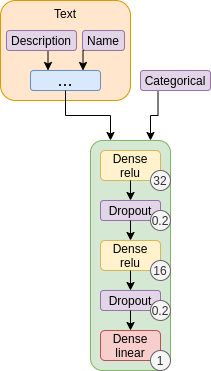
\includegraphics[
		height=6cm,
		keepaspectratio,
	]{modelTemplate.png}
	\caption{Template del modello con numero di neuroni e rate di dropout cerchiati}
	\label{fig:modeltemplate}
\end{figure}

% todo: mettere le performance nella sezione dopo
% todo: immagine del modello

% parlare di quanto tempo richiedono le 10 epoche.
% del numero dei parametri del modello.
% di quanti neuroni hanno i layers e perchè (magari fare una prova con vari
% valori bassi e aumentarli senza esagerare fino a raggiungere le performance sopra)
% parlare di qualche altro parametro? di training del modello?

\subsection{Rappresentazione del Testo}
% todo parlare della dimensionalità. di cosa è un dizionario

Sono stati valutati diversi approcci per il trattamento del testo partendo da
modelli semplici come \textit{Bag of Word} fino ai più recenti ed efficaci come \textit{BERT}.

\subsubsection{Bag of Word}
% todo: dire qualcosa della dimensionalità di bow e tf idf?
Il modello bag-of-words permette di rappresentare il testo, come una sorta di
"borsa" di parole dove per ogni "documento", o in
questo caso per ogni \textit{name} o \textit{item\_description}, viene creato un
vettore contenente il numero di occorrenze di ciascuna parola del vocabolario
nel documento; di conseguenza questi vettori avendo cardinalità pari alla
dimensione del vocabolario sono generalmente sparsi in quanto alle parole assenti
dal documento corrisponde il valore 0.
Regole grammaticali e l'ordine delle parole non sono rappresentabili
tramite questa tecnica \cite{manning_raghavan_schutze_2008}.

Ritornando al modello, per quanto riguarda Bag of Words i vettori delle feature
testuali sono forniti in input direttamente al primo layer denso allo stesso
modo delle variabili non testuali.

\subsubsection{Tf-Idf}\label{section-tfidf} Tf-Idf (Term frequency-Inverse
document frequency) \cite{manning_raghavan_schutze_2008} è una misura volta a
rappresentare l'importanza di una parola rispetto al documento che la contiene
in rapporto all'importanza della stessa nell'intera collezione di documenti;
segue la definizione.% (corpus). ?
% todo: va bene parlare di documenti? vogliamo addattare più al nostro dataset?

\begin{equation}
\label{eq:tf}
   tf_{t,d} = \frac{n_{t,d}}{|d|} 
\end{equation}
\\
\begin{equation}
\label{eq:idf}
   idf_{t} = \log \frac{|D|}{|\{d: t \in d\}|} 
\end{equation}
\\
\begin{equation}
\label{eq:tf-idf}
    Tf\mbox{-}Idf_{t,d} = tf_{t,d} \cdot idf_t
\end{equation}

Dove $t$ indica il termine, $d$
indica il documento, $n_{t,d}$ la frequenza assoluta di t in d, $D$ l'insieme
dei documenti, $|d|$ il numero di termini in $d$ e $|D|$ il numero di documenti.

Per Tf-Idf come approccio di rappresentazione del testo si vuole indendere un
approccio simile a Bag of Word i cui vettori, anzichè contenere semplicemente il
numero di occorrenze della parola, ne contengono il valore Tf-Idf
(\ref{eq:tf-idf}).

Per quanto riguarda il modello è stato utilizzato allo stesso modo di Bag
of Words. 

% todo dobbiamo parlare del layer di concatenazione?

% abbiamo dovuto aumentare i parametri rispetto alle categoriche?

\subsubsection{Word Embedding}

Le precedenti tecniche sono semplici da realizzare, robuste e funzionali per
numerosi task. Tuttavia sono poco performanti in alcune applicazioni poiché
trattano le parole come unità atomiche, senza apprenderne relazioni complesse
ad esempio di similarità o causalità.
% nel senso che non si capisce se una parola è simile ad un altra e non si hanno
% relazioni del tipo una parola segue sempre l'altra. todo: è giusto dire
% causalità?

Con lo sviluppo delle tecniche di Machine Learning si sono diffusi i cosiddetti
\textit{word embedding} che consentono di rappresentare parole per mezzo di
vettori densi e di lunghezza fissa \cite{almeida2019word}, fornendo di
conseguenza una rappresentazione più efficiente rispetto alla \textit{Bag of
words}.

Inoltre questi vettori sono in grado di apprendere relazioni semantiche e
sintattiche tra le parole \cite{mikolov2013efficient}.

% word embedding di keras
\subsubsection{Keras Embedding Layer}

Keras fornisce un implementazione di embedding sotto la forma di layer neurale e
ne rende quindi possibile l'addestramento insieme al resto del modello.

% % todo dire dopo questa cosa con glove
% Offre inoltre la possibilità di fissare il valore dei pesi semplificando
% l'integrazione con modelli pre-allenati.

Ritornando al modello, è necessario codificare le frasi di input sotto forma di
vettori di interi, a tal proposito keras fornisce la classe
\textit{tf.keras.preprocessing.\-text.Tokenizer}; questi vettori saranno in
seguito dati in input al modello.

Tenendo come riferimento il template in figure
\ref{fig:modeltemplate}, nella sezione che tratta il testo, precisamente in
sostituzione al box "..." sono stati aggiunti due layer embedding, uno per
\textit{Name} e uno per \textit{Item\_description}, seguiti da layer aggiuntivi
per sfruttare al meglio le informazioni degli embedding.

In particolare sono stati utilizzati layer RNN poiché risultano ottimi per
l'elaborazione di dati sequenziali, come il testo, essendo in grado di mantenere
in "memoria" informazioni sugli elementi precedenti \cite{liang2017text}; ad
esempio sono in grado di cogliere relazioni tra le parole di una stessa frase.

Nello specifico sono stati considerati layer LSTM, GRU e LSTM bidirezionali di
cui si parlerà più dettagliatamente in seguito.

Infine l'output di questi layer è stato assegnato come input al primo layer
denso come mostrato. La figura \ref{fig:kerasModel} ne mostra uno schema.


% todo conv

\begin{figure}[h!]
	\centering
	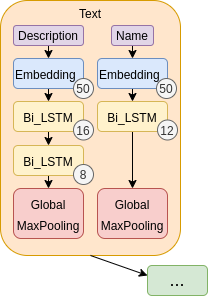
\includegraphics[
		height=5cm,
		keepaspectratio,
	]{kerasModel.png}
	\caption{Schema riassuntivo sulla gestione dei dati testuali, dove per Bi\_LSTM si intendono layer LSTM bidirezionali con dropout a 0.2 e i valori cerchiati identificano il numero di neuroni.}
	\label{fig:kerasModel}
\end{figure}

% Nel modello è stata utilizzata l'implementazione di word embedding fornita da
% Keras sotto forma di layer. La sua dimensionalità è stata impostata a 50 e to
% be continued... todo dire ciò in qualche modo. magari nei risultati

\subsubsection{GloVe}
GloVe (Global Vectors) è un modello non supervisionato in grado di costruire
word embedding a partire da statistiche globali (rispetto all'intero
corpus) di co-occorrenza delle varie parole \cite{pennington2014glove}. Sono
inoltre disponibili modelli GloVe pre-addestrati; seguono quelli valutati nel
progetto.
\begin{itemize}
	\item Wikipedia 2014 + Gigaword 5: allenato su 6 miliardi di parole e con un
	vocabolario di 400 mila parole. Fornisce vettori 50 dimensioni ed è il più "piccolo" tra i pre-addrestrati.
	\item Common Crawl: allenato su 840 miliardi di parole e con un vocabolario
	di 2.2 milioni di parole; è il più grande e fornisce vettori di 300 dimensioni.
\end{itemize}

% todo modello glove embedding keras trainable false
Per quanto riguarda il modello, trattandosi di word embedding, è stata
utilizzata la stessa architettura del modello Keras assegnando i pesi
preaddestrati e la corretta dimensionalità ai layer Embedding che sono stati impostati come non-trainabili.
% todo 50% copertura nei risultato

\subsubsection{Transformers}
% diremo che il trasform supera lstm. todo pro-cons lstm: tipo memoria,...
Il Transformer è un'architettura proposta successivamente alle RNN che vi si
contrappone evitando la ricorrenza e utilizzando esclusivamente un meccanismo di
\textit{attention} per rappresentare i rapporti di dipendenza di input e output.
Si basa su di una struttura \textit{encoder-decoder} dove l'encoder fornisce al
decoder una rappresentazione dell'input ed in seguito il decoder fornisce una
frase in output \cite{vaswani2017attention}.

% todo decidere se togliere l'anno

% BERT’s model architecture is a multi-layer bidirectional Transformer encoder
% based on the original implementation

Una delle più note architetture basata sul concetto di Transformer è
\textbf{BERT}, ovvero \textit{Bidirectional Encoder Representations from
Transformers}; si tratta di un transformer multi-layer bidirezionale, cioè 
che dato un input è in grado di apprenderne relazioni sia con input precedenti
che successivi, e che si basa esclusivamente su
 moduli encoder. Nasce al fine di fornire un modello
pre-allenato adattabile semplicemente ad un vasto range di applicazioni tramite
\textit{fine-tuning}. Tuttavia anche approcci \textit{feature-based} basati
su BERT risultano efficaci \cite{devlin2018bert}.
% todo feature based è giusto?

In questo progetto è stato utilizzata una versione più leggera e veloce ottenuta
da BERT tramite \textit{Knowledge distillation}, ovvero DistilBert
\cite{sanh2020distilbert}, con un approccio feature-based.

Ritornando al modello, occupa la stessa posizione dedicata agli embedding
(figura \ref{fig:kerasModel}), per entrambi i campi nome e descrizione.

\subsection{Training e valutazione}

\subsubsection{Dataset split}

Al fine di valutare i vari modelli più correttamente possibile il dataset è
stato suddiviso in \textit{training-set}, \textit{validation-set} e
\textit{test-set}.

\subsubsection{Valutazione dell'errore}
% loss e metriche

Per quanto riguarda le performance in termini di errore la funzione di
\textit{loss} utilizzata in fase di training è il \textit{Root Mean Squared
Logaritmic Error (RMSLE)}, in quanto è la misura scelta dalla Kaggle challenge
per confrontare le performance dei vari partecipanti. Risulta inoltre
adeguata al problema considerando il vasto intervallo dei valori dei prezzi.

Seguono la definizione e alcune osservazioni su di RMSLE e MSLE.
\\
\textit{Mean Squared Logarithmic Error (MSLE)}, essendo calcolato a partire
da un rapporto, riflette l'errore relativo e di conseguenza risulta efficace
laddove i valore assoluti presentano variazioni considerevoli.
\begin{equation}
    \frac{1}{n}
        \sum_{i=1}^{n}
            ( \log(y_i+1) - \log(\hat{y_i}+1) )^2
    =
    \frac{1}{n}
        \sum_{i=1}^{n}
            \log^2(\frac{y_i+1}{\hat{y_i}+1})
\end{equation}
\\
\textit{Root Mean Squared Logarithmic Error (RMSLE)} è la radice di MSLE.
\begin{equation}
    \sqrt{ 
        \frac{1}{n}
            \sum_{i=1}^{n}
                ( \log(y_i+1) - \log(\hat{y_i}+1) )^2
    }
\end{equation}

% todo riassumere tutto in rmsle per guadagnare spazio

% dire da qualche parte qualche altra valutaione: e.g. la computazione richiesta
% dai vari approcci

% todo numero parametri

\subsubsection{Valutazione dei costi computazionali}

Per la valutazione dei costi computazionali sono stati annotati il numero dei
parametri allenabili e non dei vari modelli, il tempo richiesto dall'allenamento
sul trainset e quello richiesto dalla predict sul testset.

È stata utilizzata la piattaforma \textit{Google Colab} abilitando l'accelerazione hardware GPU.


\subsection{Parametri di training}
% todo sono risultati?

\paragraph{Numero di neuroni:} Il numero di neuroni dei vari layer è stato
impostato ai valori mostrati nelle figure \ref{fig:modeltemplate} e
\ref{fig:kerasModel} in modo da migliorare le performance di regressione.

\paragraph{Optimizer:} Come optimizer è stato utilizzato Adam impostando il learning rate a 1e-4, in quanto il training è
risultato più stabile che con il default di 1e-3 per la maggior parte degli
approcci ad eccezione dell'Embedding Keras che ha dimostrato un comportamento
migliore con il learning rate di default.

\paragraph{Batchsize:} La batchsize è stata impostata a 256 dopo alcuni test
sperimentali.

\paragraph{Regolarizzazione:} Oltre ai layer Dropout è stato testata la
regolarizzazione L2, tuttavia non ha portato a evidenti miglioramenti ed è
quindi stata omessa. Inoltre abbiamo utilizzato l'earlystopping sull'errore del
validation con pazienza impostata a 3 epoche e in modo da ripristinare i pesi
più performanti rispetto al validation.
